\section{ALLOY MODELLING} 
The following alloy model is obtained by referring to our class diagram. Our code file has been structured by first inserting signatures, followed by facts, assertions and predicates.
The complete code file is available on github. The results of our analysis, namely the generated worlds, are available at the end of this section.

\subsection{Signatures}
\begin{figure}[h!]
	\centering
	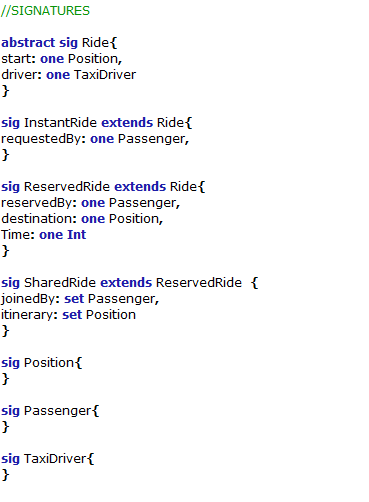
\includegraphics[height=0.75\textwidth]{Sig}
\end{figure}

\newpage

\subsection{Facts}
\begin{figure}[h!]
	\centering
	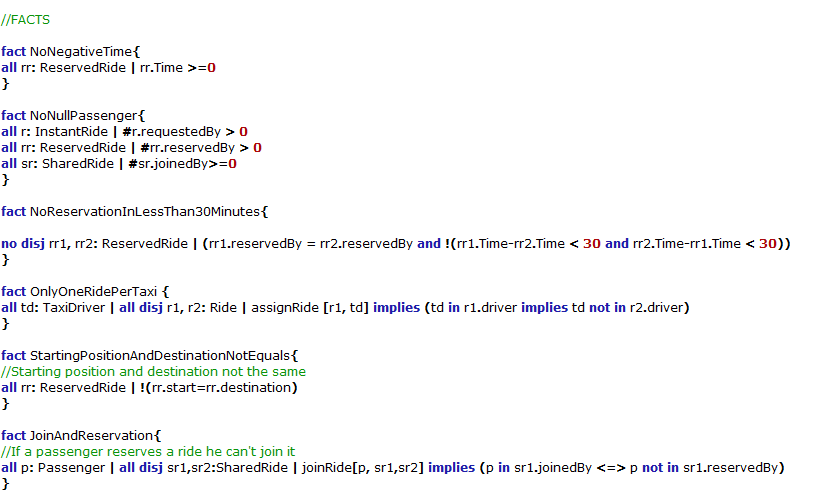
\includegraphics[height=0.65\textwidth]{Facts}
\end{figure}

\newpage
\subsection{Assertions}
\begin{figure}[h!]
	\centering
	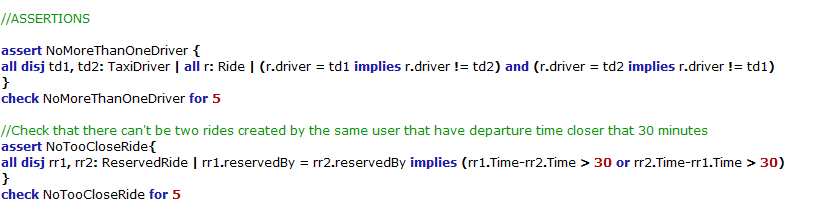
\includegraphics[width=1.3\textwidth]{Assert}
\end{figure}

\newpage
\subsection{Predicates}
\begin{figure}[h!]
	\centering
	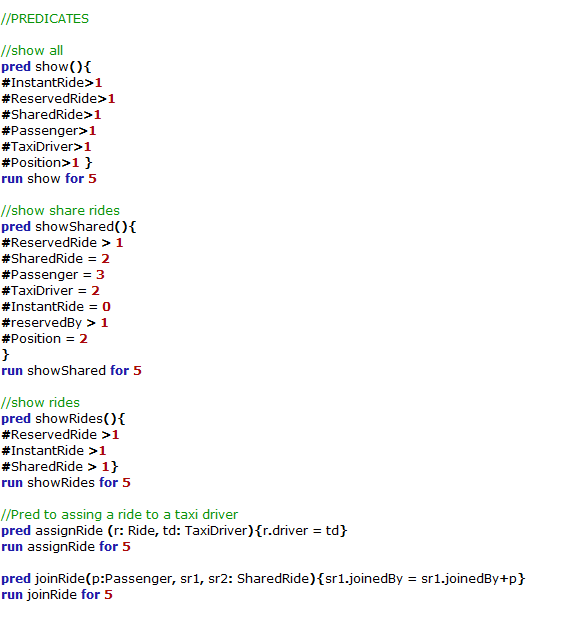
\includegraphics[width=\textwidth]{Predicates}
\end{figure}

\newpage

\subsection{Generated Worlds}
\subsubsection{Show Predicate}
\begin{figure}[h!]
	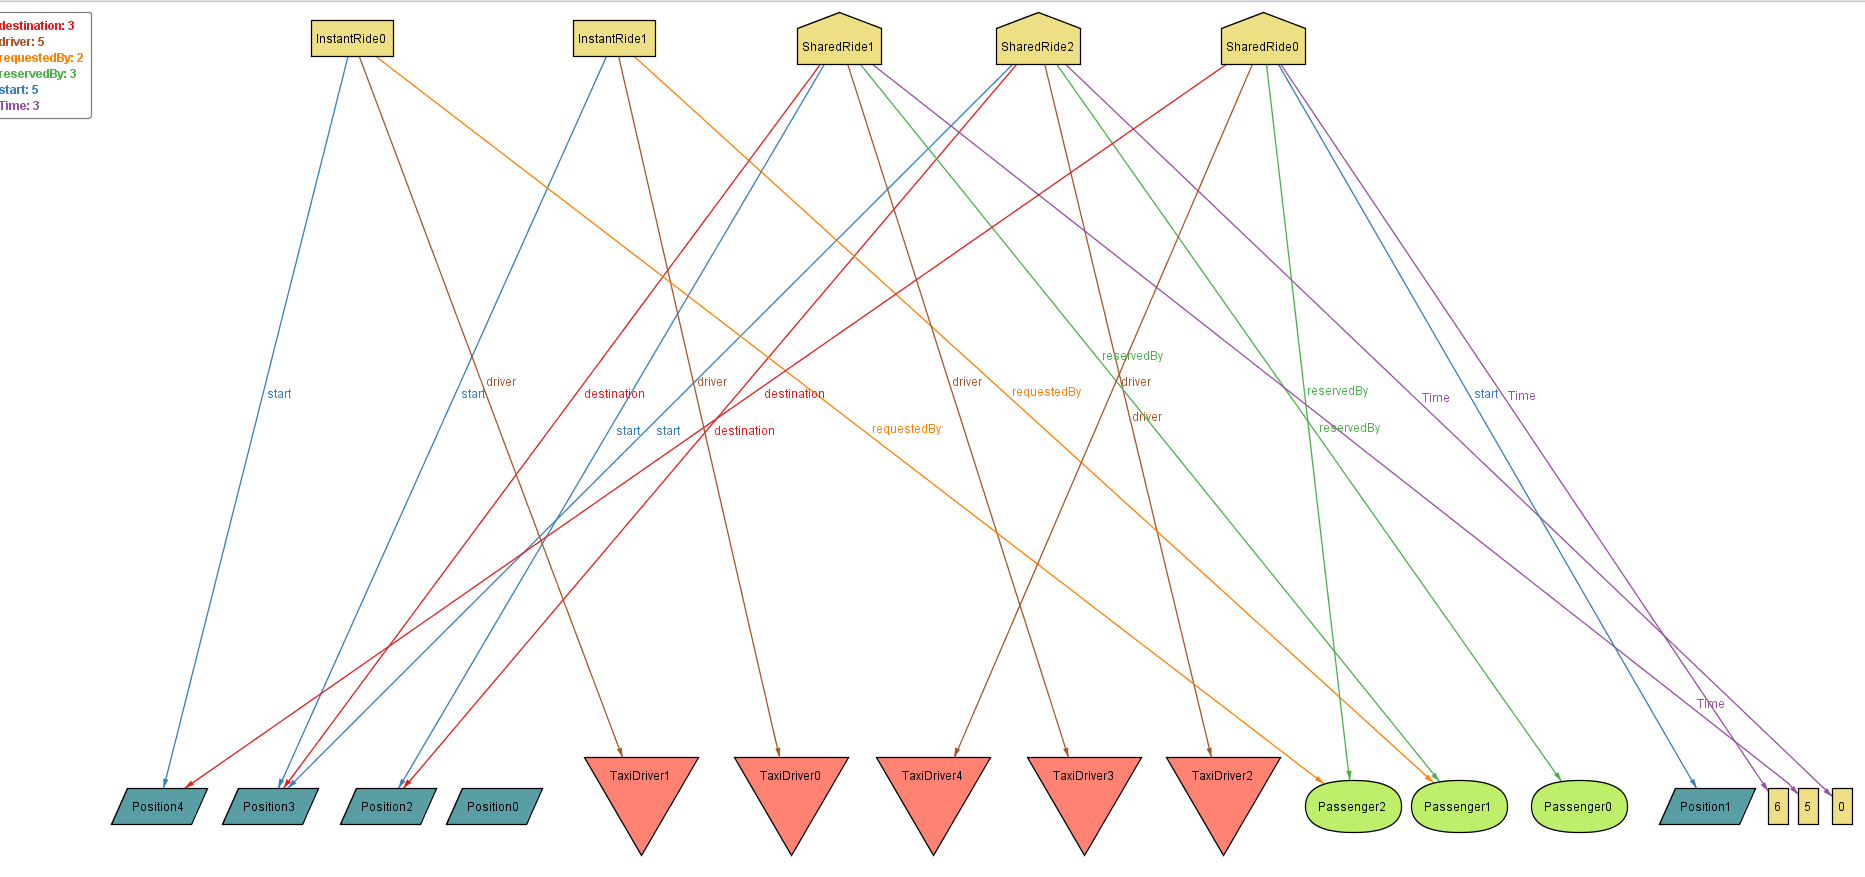
\includegraphics[width=\textwidth]{Show}
\end{figure}
\newpage

\subsubsection{Show Shared Predicate}

\begin{figure}[h!]
	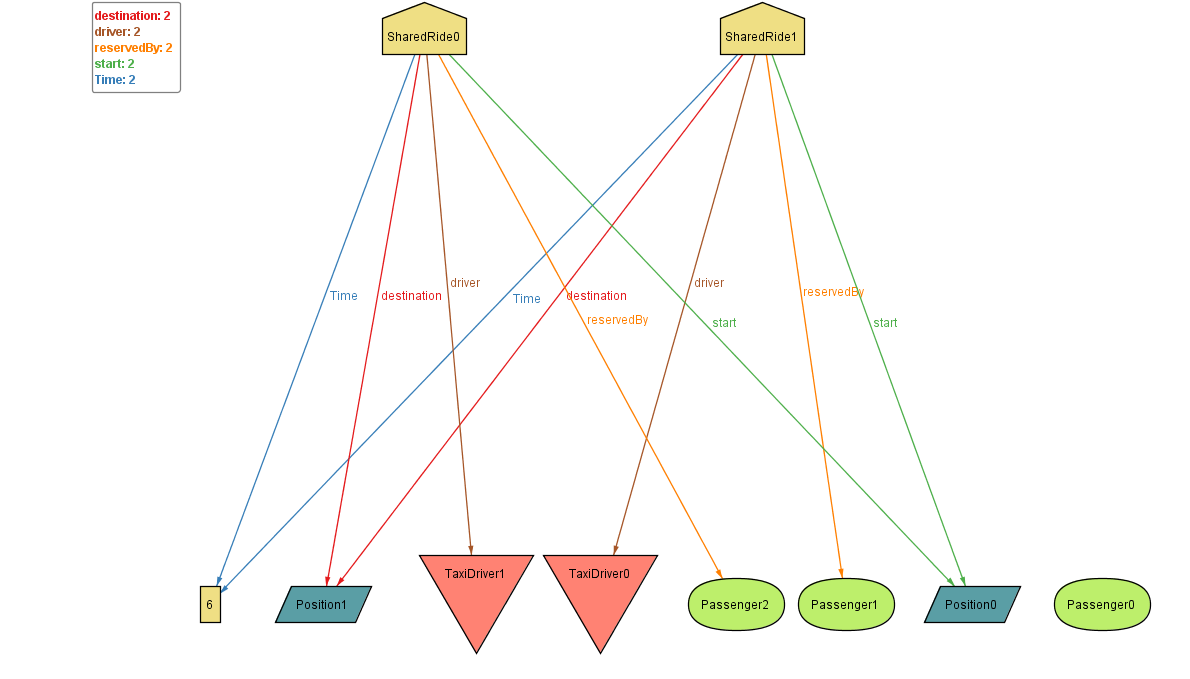
\includegraphics[width=\textwidth]{ShowShared}
\end{figure}
\newpage

\subsubsection{Show Rides Predicate}
\begin{figure}[h!]
	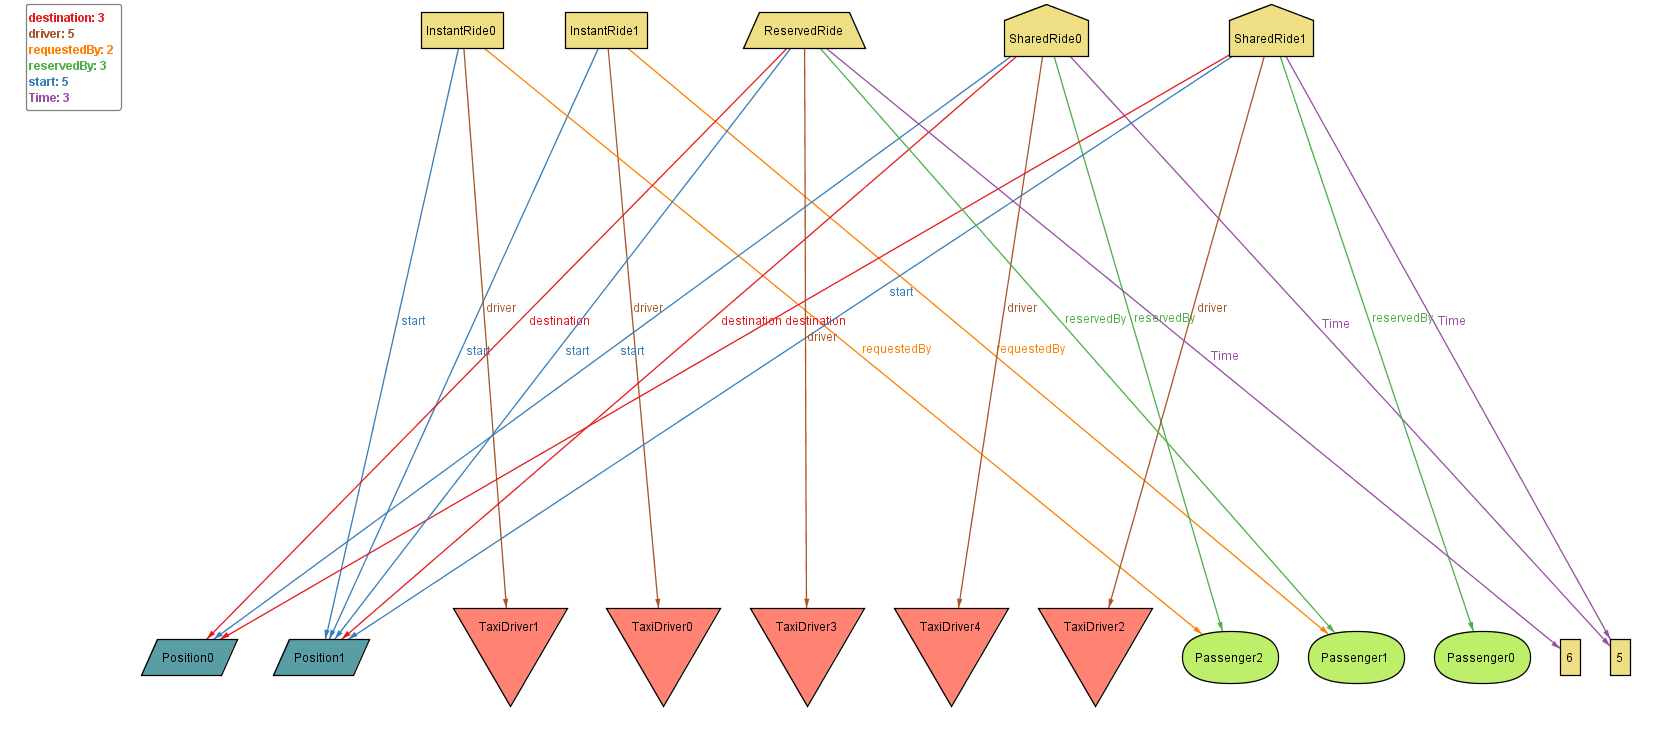
\includegraphics[width=\textwidth]{ShowRides}
\end{figure}
\newpage
